% Nejprve uvedeme tridu dokumentu s volbami
\documentclass[slovak,master,public,dept460,male,cpdeclaration,oneside]{diploma}
% Dalsi doplnujici baliky maker
\usepackage{subfig}		% makra pro "podobrazky" a "podtabulky"
\usepackage{tikz}		% makra pro kresleni
\usepackage{amssymb}
\usepackage{amsmath}
\usepackage{float}
\usepackage{graphicx}
\usepackage[utf8]{inputenc}
\usepackage{color}

% Zadame pozadovane vstupy pro generovani titulnich stran.
\ThesisAuthor{Veronika Uhrová}

\CzechThesisTitle{Analýza emailové komunikace}

\EnglishThesisTitle{Analysis of Email Communication}

\SubmissionDate{\now}

% Pokud nechceme nikomu dekovat makro zapoznamkujeme.
\Thanks{Moje poďakovanie patrí predovšetkým doc. Milošovi Kudělkovi, Ph.D. za odborné konzultácie a vedenie mojej diplomovej práce.}

% Zadame cestu a jmeno souboru ci nekolika souboru s digitalizovanou podobou zadani prace.
% Pokud toto makro zapoznamkujeme sazi se stranka s upozornenim.
\ThesisAssignmentImagePath{Figures/Assignment}

% Zadame soubor s digitalizovanou podobou prohlaseni autora zaverecne prace.
% Pokud toto makro zapoznamkujeme sazi se cisty text prohlaseni.
\AuthorDeclarationImageFile{Figures/AuthorDeclaration.jpg}

\ThesisAccessRestriction{Zde vložte text dohodnutého omezení přístupu k Vaší práci, chránící například firemní know-how. Zde vložte text dohodnutého omezení přístupu k Vaší práce, chránící například firemní know-how. A zavazujete se, že:
\begin{enumerate}
\item podle \textsection{} 5 o práci nikomu neřeknete,
\item po obhajobě na ni zapomenete a
\item budete popírat její existenci.
\end{enumerate}
A ještě jeden důležitý odstavec. A ještě jeden důležitý odstavec.
A ještě jeden důležitý odstavec. A ještě jeden důležitý odstavec.
A ještě jeden důležitý odstavec. A ještě jeden důležitý odstavec.
Konec textu dohodnutého omezení přístupu k Vaší práci.}

% Zadame soubor s digitalizovanou podobou souhlasu spolupracujici prav. nebo fyz. osoby.
% Pokud toto makro zapoznamkujeme sazi se cisty text souhlasu.
\CooperatingPersonsDeclarationImageFile{Figures/CoopPersonDeclaration.jpg}

\CzechAbstract{Toto je slovenský abstrakt...}

\CzechKeywords{typografie, \LaTeX, diplomová práca}

\EnglishAbstract{This is English abstract...}

\EnglishKeywords{typography, \LaTeX, master thesis}

\AddAcronym{MUA}{Mail User Agent}
\AddAcronym{MTA}{Mail Transfer Agent}
\AddAcronym{IMAP}{Internet Message Access Protocol}
\AddAcronym{XML}{eXtensible Markup Language}
\AddAcronym{SSRM}{Structural social role mining framework}




% Zacatek dokumentu
\begin{document}

% Nechame vysazet titulni strany.
\MakeTitlePages

% Pokud mame v zaverecne praci vypisy kodu, jinak odstranit.
\lstlistoflistings

% A nasleduje text zaverecne prace.
\section{Úvod}

\subsection{Motivácia}
S cieľom uľahčiť používanie emailov a prebádať podnikateľský potenciál emailov, dolovanie emailov, ktoré používa aj techniky zberu dát, dosiahlo pozoruhodný pokrok v oblasti výskumu a aj v praxi. Emaily teda možno považovať za zmiešanú štruktúru obsahujúcu aj textové údaje, ako aj ľudské, sociálne, organizačné vzťahy.


\textbf{Obsah emailu ako textové a netextové dáta} Emaily sú písané viac stručne ako väčšina ostatných dokumentov, často obsahujú hovorové výrazy a abreviácie, ktoré sa nenachádzajú v bežných slovníkoch, preto štandartné techniky dolovania textov nemusia byť efektívne, pri práci s emailovými dátami.

Emaily tiež obsahujú bohatšie typy dát, ako napríklad URL linky, HTML tagy alebo obrázky. Nniektoré štúdie jednoducho zjednodušia tieto netextové dátové vstupy v štádiu predpripravovania dát - vymažu ich a ďalej pracujú len s textovými dátami. Tieto netextové dáta však môžu byť užitočné iných oblastiach, ako napríklad detekcia spamu. 


\textbf{Emaily reprezentujúce ľudské sociálne organizačné vzťahy} Emailová aktivita sama o sebe reprezentuje bohaté ľudské sociálne a organizačné vzťahy, ktoré spájajú ľudí do komunít a komplexných sysémov. Porozumenie organizačných štruktúr alebo vzťahov naprieč ľudmí v organizácii môže byť veľmi užitočné aj v reálnom živote. 
Hlavné problémy, ktoré sú investigované v analýze mailov sú detekcia spamu, kategorizácia emailov, analýza kontaktov, analýza vlastností emailových sietí a vizualizácia emailov.



\section{Súvisiace práce}

Pre odhaľovanie vzťahov medzi ľuďmi, skupina a organizáciami z emalových sietí boli aplikované mnohé techniky a modely analýzy sociálnych sietí. Mnoho štúdií použilo maily spoločnosti \textit{Enron} kvôli nedostatku dostupných veľkých súborov. 


Napríklad Diesner, Carley a Frantz v \cite{3} zkonštruovali z mailovej komunikácie spoločnosti Enron orientovaný graf zo vzťahu odosielateľ-príjemca, kde hrany boli vážené frekvenciou mailov, ktoré si medzi sebou poslali v čase. Potom aplikovali techniky analýzy sociálnych sietí. V práci popísali, ako vylepšili originálnu sadu a súčasné zistenia ich investigáciou vďaka analýze sociálnych sietí. Skúmajú dynamiku, štruktúru a vlastnosti organizačnej komunikačnej siete ako aj charakteristiky a vzory komunikačného správania zamestnancov z rôznych organizačných levelov. Zistili, že počas obdobia krízy sa komunikácia medzi zamestnancami stala viac rôznorodejšia v súvislosti so zavedenými kontaktami a formálnymi rolami. Taktiež počas obdobia kríz, predtým nekomunikujúci zamestnanci sa začali zapájať do vzájomného rozhovoru, takže interpersonálna komunikácia bola intenzívnejšia a sieť sa tým rozširovala. Tieto zistenia poskytli cenný pohľad do organizačnej krízy reálneho sveta, čo môže byť ďalej využité pre validáciu alebo tvorbu teórií a dynamických modelov organizačných kríz a tým to vedie k lepšiemu porozumeniu základných príčin organizačných kríz v organizáciách.


Xiaoyan Fu v \cite{2} prezentoval rôzne metódy pre vizualizáciu emailových sietí. Vizualizácia objavuje komunikačné vzory medzi rôznymi skupinami, zobrazuje centrálnu analýzu s dôrazom na významné uzly.
V práci zkonštruovali 2D vizualizáciu temporálnej emailovej siete, ktorá analyzuje vývoj emailových vzťahov, ktoré sa menia v priebehu času a zobrazenie prostredia pre nájdenie sociálnych kruhov odvodených od siete. Každá metóda bola vyhodnotená s rôznymi datasetmi od výskumnej orgnizácie. Taktiež rozšírili ich metódu pre vizuálnu analýzu siete emailových vírusov.

Ďalej Chapanond, Krishnamoorthy, Yener v \cite{4} použil sieťové metriky a spektrálnu analýzu k analýze či už orientovaného alebo neorientovaného grafu emailov, ktorý skonštruoval zmenou prahovej hodnoty (napr. počtom vymenených emailov medzi užívateľmi). Ich výskum je postavený na vytvorení emailového grafu a štúdiu jeho vlatností či už pomocou teórie grafov alebo technikami spektrálnej analýzy. Grafová teoretická analýza zahŕňa výpočet niekoľkých grafových metrík, ako napríklad rozdelenie podľa stupňov, priemerný pomer vzdialeností, zhlukovací koeficient alebo kompaktnosť emailového grafu. Hodnoty metrík v dátovej sade emailov spoločnosti Enron porovnali aj s inými emailovými dátami. 

Jednou z univerzálnejších prác je aj práca autorov Guanting Tang, Jian Pei, and Wo-Shun Luk \cite{1}. Je to stručný prehľad hlavných výskumných snáh o analýzu mailov a popis metód, ktoré sa pri tejto analýze používajú. Nie len čo sa týka analytických alebo implemetnačných úloh, ale aj nástrojov, ktoré nám pri analýze vedia pomôcť. Aby zdôraznili rozdiely medzi analýzou mailov a bežnou analýzou textu, organizujú prieskum do piatich ťažších úloh a to:  detekcia nevyžiadanej pošty, kategorizácia emailov, analýza kontaktov, analýza vlastností emailovej siete a vizualizácia emailov. Tieto úlohy sú vlastne začlenené do rôznych spôsobov používania emailov. Systemaicky preskúmavajú bežne používané techniky a tiež budujú diskusiu o dostupných softwarových nástrojoch.

Na rozdiel od ostatných prác, Afra Abnar, Mansoureh Takaffoli, Reihaneh Rabbany, Osmar R. Zaıane \cite{9} definovali vlastnú metodiku pre analýzu sociálnej siete a definovali \textit{Structural social role mining framework}, ktorý je navrhnutý pre identifikáciu štrukturálnych rolí, pre identifikáciu zmien v sieti a analýzu dopadu zmien na sieť. Definujú základné sociálne roly v sieti a navrhujú metodológie pre ich identifikáciu. Pre identifikáciu týchto rolí využívajú klasické prostriedky analýzy sociálnych sietí a tiež navrhujú nové metriky zahrňujúc napríklad Betweenness centrality založenú na komunitách. Z tejto práce som vychádzala pri pomenovaní rolí zo siete a implementovala techniky pre ich identifikáciu.

Ďalšou prácou, ktorou som sa inšpirovala bola práca autorov Kudělka, Horák, Zehnalová \cite{10}, ktorá prezentuje analytický nástroj, ktorý bol vztvorený pre analýzu hlbších vzťahov v emailových dátach. Tieto vzťahy zahrňujú vzťahy založené na interakcii viacerých užívateľov v tíme. Analytické metódy popísané v práci sú založené na dvoch faktoroch. Prvým faktorom je kontext, čo je skupina viacerých užívateľov v kombinácii so slovami použitými v komunikácii. Druhým faktorom je časový interval, v ktorom bola začatá komunikácia. Práca prezentuje metódy pre váženie komunikácií, užívateľov a vzťahov, ako aj metód pre hľadanie komunít asociovaných so špecifickým kontextom. Inšpirovala som sa hlavne tým, ako je v práci definovaná konverzácia, čo popisujem v kapitole: (doplniť!!!!)

\section{Definície a klasifikácie}
V tejto kapitole popisujem všetky teoretické pojmy a metódy, ktoré v tejto práci spomínam a používam. V tejto kapitole budem používať matematické názvy podľa kontextu, v ktorom sa budem nachádzať.

\subsection{Graf}
\begin{itemize}

\item \textbf{Neorientovaný graf}

Neorientovaným grafom rozumieme usporiadanú dvojicu \textit{G = (V, E)}, kde \textit{V} je neprázdna množina \textit{vrcholov} a \textit{E} je neprázdna množina \textit{hrán} - množina (niektorých) dvojprvkových podmnožín množiny \textit{V}.

\begin{figure}[H]
\centering
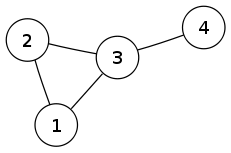
\includegraphics[width=7cm,height=4.5cm]{figures/neorientovany}
\caption{Neorientovaný graf}
\end{figure}

\item \textbf{Orientovaný graf}

Orientovaným grafom rozumieme usporiadanú dvojicu \textit{G = (V,E)}, kde V je množina \textit{vrcholov} a množina orientovaných \textit{hrán} je $E \subseteq  V \times V$. 

\begin{figure}[H]
\centering
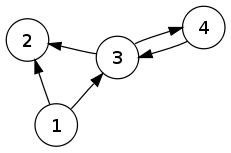
\includegraphics[width=7cm,height=4.5cm]{figures/orientovany}
\caption{Orientovaný graf}
\end{figure}

\newpage
\item \textbf{Súvislosť grafu}

Hovoríme, že vrchol \textit{v} je \textit{dosiahnuteľný} z vrcholu \textit{u}, ak v grafe existuje sled z vrcholu \textit{u} do vrcholu \textit{v}.

Graf nazveme \textit{súvislý}, ak pre každé dva vrcholy \textit{u, v} je vrchol v dosiahnuteľný z vrcholu u. V opačnom prípade je graf \textit{nesúvislý}.

\item \textbf{Úplný graf}

Úplný graf na ${n}$ vrcholoch je neorientovaný graf, ktorý má hranu medzi každými dvoma vrcholmi. Počet jeho hrán je ${m = n * ( n - 1) / 2}$.

\item \textbf{Stupeň vrcholu}

Stupeň vrcholu je počet vrcholov spojených s týmto vrcholom hranou, inými slovami: počet jeho susedov. V orientovanom grafe sa ešte rozlišuje vstupný a výstupný stupeň vrcholu podľa toho, koľko hrán z vrcholu vychádza alebo do neho vchádza.

\item \textbf{Cesta}

Cesta je postupnosť vrcholov v grafe taká, že medzi každými dvoma vrcholmi cesty je hrana a vrcholy sa neopakujú. V orientovaných grafoch sa ešte rozlišuje smer cesty, pričom orientácia hrán je stále rovnaká. Dĺžka cesty je počet hrán, ktoré obsahuje.

\item \textbf{Uzavretá cesta}

Uzavrená cesta, kružnica v neorientovanom a cyklus v orientovanom grafe, je cesta, ktorá začína a končí v rovnakom uzle.

\item \textbf{Komponenta grafu}

Komponenta grafu je súvislá časť grafu a medzi vrcholmi z rôznych komponent neexistuje žiadna hrana.

\end{itemize}


\section{Sociálna sieť}

Sociálna sieť je množina sociálnych subjektov (uzly siete, spravidla jednotlivci alebo organizácie),
ktoré sú prepojené jedným, alebo viacerými špecifickými druhmi vzájomnej závislosti, ako sú príbuzenstvo, priateľstvo, vzájomnosť, vízie, odpor, konflikt, obchod a pod.
Sociálna sieť z pohľadu teórie grafov je definovaná ako graf G(V, E), kde V je množina entít
(uzlov) a E je množnina vzťahov (hrán) medzi týmito entitami.

Entity grafu môžu byť rôzne (zákazníci, jednotlivci, webové stránky, bankové účty, creditné karty,
produkty). Nie je pravidlom, že len sociálna sieť ako ju pozná mnoho ľudí je sociálnou sieťou aj formálne. Prvky sociálnej siete môže ma napríklad aj skupina spolupracujúcich ľudí. 

\subsection{História sociálnych sietí}

Pod pojmom sociálna sieť si väčšina ľudí v dnešnej dobe predstaví služby ako \textit{Facebook, Twitter} a pod. Tento pojem ale vznikol dlho pred vznikom internetu a dnešných sociálnych sietí. Prívlastok sociálny, ktorý sa v dnešnej dobe často vynecháva, je dôsledkom pôvodu analýzy sociálnych sietí. V druhej polovici 20. storočia sa simultánne v rôznych oblastiach skúmania vzťahov a chovania objavil nový pohľad na vzťahy medzi sociálnymi jednotkami a to ako na sieť, graf. Preto prví predstavitelia analýzy sociálnych sietí boli pôvodne sociológovia alebo psychológovia (napríklad Moreno, Cartwright, Newcomb, Bavelas) a antropológovia (Barnes,Mitchell). Prvé použitie termínu "sociálna sieť" sa pripisuje Barnesovi (1954).

V 30. rokoch 20. storočia psychiater Moreno rozvíjal sociometriu, predchodcu dnešnej analýzy sociálnych sietí. Vypytoval sa ľudí na priateľské vzťahy a skúmal, ako tieto vzťahy ovplyvňujú ich chovanie. Potom vynašiel (sám to tvrdill) tzv. \textit{sociogram}, čo je diagram reprezentujúci ľudí ako body a vzťahy medzi ľuďmi ako úsečky, teda dnešnú sociálnu sieť. Tento pojem sa ale začal používať až neskôr. Pomocou neho hľadal výrazné a izolované osoby v spoločnosti.

Zhruba o 20 rokov neskôr antropológ Barnes začal skúmať, ako ovplyvnia vzťahy medzi ľuďmi nielen jednotlivcov, ale aj spoločnosť ako celok a zameral sa na štúdium skupín, komunít. Na práci Barnesa a jeho spolupracovníkov naviazala na Univerzite na Harvarde skupina vedená Harrisom Whitom. Tá začala budovať matematickú teóriu okolo dôležitejšcíh pojmov zo sociálnych vied a umožnila tieto javy matematicky vyjadriť, merať a modelovať.

V druhej polovici 20. storočia sa rozšírilo povedomie o sociálnych sieťach a metódy sa začali používať aj v ďalších oboroch ako ekonómia, biológia, doprava atd.

\subsection{Analýza sociálnych sietí}

Analýza sociálnych sietí je interdisciplinárna veda s koreňmi v sociológii, psychológii,
štatistike a teórie grafov. Analýza sociálnej siete chápe sociálnu sieť ako systém prepojenia uzlov (individuálnych aktérov) prostredníctvom hrán (ich vzťahov). Možno teda povedať, že nadväzuje na matematickú teóriu grafov a metódy sieťovej analýzy. Výsledkom analýzy môže teda byť mapa graficky znázorňujúca všetky prvky skúmaného sociálneho systému a ich vzťahy (resp. vybrané charakteristiky jednotlivých vzťahov vyjadrené vhodným spôsobom graficky). Charakteristikou môže byť napríklad vzájomná sympatia či antipatia alebo pravidelná vzájomná komunikácia alebo spolupráca.


Analýza sociálnych sietí vystupuje napríklad ako základná technika v rámci modernej sociológie,
antropológie, sociálnej lingvistiky, geografie, sociálnej psychológie, ekonómie a biológie
rovnako ako populárna téma pre výskum. 

\subsection{Komunity v sociálnych sieťach}

Sociálne siete sú riedke grafy zložené z hustých podgrafov. Tieto husté podgrafy sú nazývané
komunity. Najčastejšia definícia komunity: \textit{Komunita je zhluk uzlov, kde počet vnútorných hrán v komunite je väčší ako počet vnokajších hrán – mimo komunity}. \cite{8}

Algoritmy pre dolovanie komunít sú založené na spojoch medzi uzlami, ktoré naznačujú
spojenie dvoch entít. Napr. SCAN (Structural Clustering Algorithm for Networks) je metóda
pre detekciu komunít v súvislosti na to, ako uzly zdieľajú svojich susedov len s ohľadom na
priame spojenie. Teda ak sú dva uzly spojené a tiež zdieľajú rozumné množstvo ich susedov,
patria do rovnakej komunity.


\begin{figure}[H]
\centering
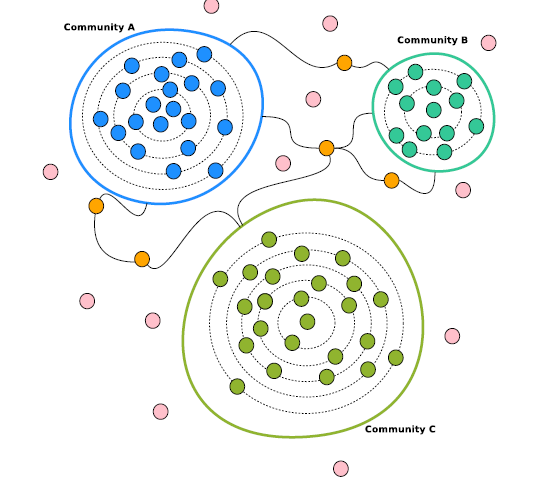
\includegraphics[width=12cm,height=10cm]{figures/comunities}
\caption{Sieť s viacerými komunitami}
\end{figure}


\subsection{Detekcia komunít}
Detekcia komunít je proces identifikácie zhlukov uzlov siete silne prepojených medzi sebou a menej silne prepojených so zvyškom siet. Detekcia komunít v grafoch má za cieľ identifikovať moduly a ich prípadnú hierarchickú organizáciu.


\section{Emailová komunikácia}
\subsection{Stručná história emailu}
Za počiatky emailovej komunikácie možno považovať priližne rok 1965, kedy bola správa prenášaná medzi sálovými počítačmi pracujúcich v režime zdieľania času na univerzite \textit{Massachusetts Institute of Technology}.

Od tejto doby preša emailová komunikácia značným vývojom. Emaily, tak ako ich poznáme dnes, sú definované štandartom špecifikácie RFC2822 a sú prenášané pomocou komunikačných protokolov. 


\subsection{Štruktúra emailu}
Každý email sa skladá z dvoch častí - z tzv. hlavičky \textit{(header)} a tela emailu \textit{(body)}.

Hlavička emailu je generovaná automaticky pri vytvorení emailu a sú do nej postupne vkladané informácie zo serverov, cez ktoré správa prechádza (tzv. MTA). Pre bežných užívateľov sú z hlavičky najdôležitejšie tieto údaje: predmet správy, čas odoslania, emailová adresa odosielateľa a prijímateľa. Ostatné údaje emailoví klienti (označovaní tiež ako MUA \footnote{MUA - Mail User Agent, program, ktorý používa užívateľ na rozosielanie a prijímanie emailov (napr. Outlook), tento program komunikuje s MTA (Mail Transfer Agent), ktorý sa stará o prenos emailov v prostredí verejnej siete Internet.}) väčšinou nezobrazujú.


Pri vytváraní emailu emailovým klientom sú väčšinou do hlavičky vložené tieto záhlavia:

\begin{itemize}
\item \textbf{Date} - aktuálny čas počítača, ktorý vložil záhlavie
\item \textbf{From} - adresa odosielateľa
\item \textbf{Cc} - špecifikuje ďalších adresátov
\item \textbf{Bcc} - umožňuje rozosielanie správy medzi viacerých adresátov
\item \textbf{Priotity} - priorita emailu, interpretácia sa líši vzhľadom k MUA
\item \textbf{Reply-To} - špecifikuje adresu, na ktorú je zaslaná prípadná odpoveď
\item \textbf{Subjekt} - predmet správy daný užívateľom
\item \textbf{To} - udáva adresu príjemcu správy
\item \textbf{Message-Id} unikátny identifikátor, ktorý je priradený MTA
\end{itemize}





Telo emailu obsahuje samotné dáta určené pre adresáta. 


\subsection{Emaily v súčasnosti}
Emaily teda existujú už niečo cez 50 rokov, ich popularita je však stále veľká vďaka ich efektivite, extrémne nízkym nákladom a kompatibilite s množstvom typov zariadení. Ako jedna z najrozšírenejších typov komunikácie v dnešnej dobe, emaily sú široko rozšírené v každodennom živote. Napríklad, spolupracovníci diskutujú prácu cez emaily, priatelia zdieľajú sociálne aktivity a skúsenosti aj cez emaily alebo veľké spoločnosti distribuujú reklamy práve pomocou emailov.


\section{SSRM - Framework pre detekciu štrukturálnych rolí v sociálnych sieťach}

Afra Abnar, Mansoureh Takaffoli, Reihaneh Rabbany, Osmar R. Zaıane \cite{9} definovali \textit{Structural social role mining framework}, ktorý je navrhnutý pre identifikáciu štrukturálnych rolí, pre identifikáciu zmien v sieti a analýzu dopadu zmien na sieť. Definujú základné sociálne roly v sieti(menovite Leader, Outermost, Mediator, Outsider). 

\subsection{Rola v kontexte SSRM}
\textit{Sociálna rola} je síce základný sociologický pojem, ale stále neexistuje žiadny konsenzus v jej definícii. Podľa SSRM je rola je považovaná za pozíciu jednotlivca v spoločnosti.
 Informácie o sociálnej sieti sú kategorizované do štrukturálnych a neštrukturálnych vlastností. Štrukturálne vlastnosti sú príbuzné ku konštrukcii grafu ako sú spojenia entít (hrany), štruktúra susedov a pozícia entity v tejto štruktúre. Ale neštrukturálne vlastnosti sú ostatné informácie, ktoré neodrážajú konštrukciu grafu ako atribúty entít a spojení. SSRM definuje rolu v sieti ako: Rola entity v sieti je to, ako sa entita správa voči ostatným a jej vplyv na atribúty a štruktúry ostatných entít.


\subsection{Roly definované v SSRM}
Ľudské siete sú vnútorne zložené z viacerých komunít. V sociálnej sieti s viacerými komunitami, vlastnosti uzlov kolíšu podľa toho, či je existencia komunít dostatočná alebo zanedbateľná. Z pohľadu sociálnej siete, uzol môže byť centrom celej siete, ale nie centrom v jeho komunite. SSRM sa teda zameriava na štúdium sociálnych sietí s predpokladom existencie komunít v sieti, ako jej základnej črty.

V sociálnych sieťach môžu byť komunity explicitné alebo implicitné. Explicitné komunity sú postavené nezávisle na jej členoch a sú založené na množine pravidiel. V tomto prípade, ľudia sa stanú členmi tejto komunity častejšie až po zformovaní komunity. Zamestnanci firmy alebo študenti sú príkladom dvoch explicitných komunít. Zatiaľ čo formácia implicitných komunít ťažko závisí na jej členoch a spojeniach. Tým pádom neexistuje žiadna externá podmienka na vybudovanie implicitnej komunity. Implicitné komunity sú postavené postupne ako sa ľudia spoločne stretávajú. Napríklad, skupina priateľov, v ktorej nie je žiadne pravidlo pre správanie sa jednotlivcov, je príklad implicitnej komunity. V oboch prípadoch explicitnej aj implicitnej komunity, by mali existovať aj špeciálny jednotlivci, ktorí tieto komunity manažujú a kontrolujú. Napríklad v školskej triede je to učiteľ alebo inštruktor. Pre firmu to je manažér vo vedení a pre skupinu priateľov je to zase človek, ktorého komunikačné schopnosti prinášajú ďalších členov alebo posilňujú vzťahy medzi tými stálymi. Títo dôležitý jednotlivci sú ešte viac výrazný, keď je komunita obrovská.


Podľa toho SSRM framework definuje pre jednotlivcov v sociálnej sieti určité roly podľa ich vzťahov a pozícií v komunitách až po ich interakcie s ostatnými jednotlivcami. Z perspektívy komunít, v sieti existujú jednotlivci niekoľkých typov:

\begin{itemize}
\item so žiadnym vzťahom ku nejakej komunite
\item so spojením s viacerými komunitami
\item dôležitý členovia komunity
\item bežný členovia komunity, ktorí formujú väčšinu
\item nedôležitý členovia komunity, ktorí nemajú na komunitu pozorovateľný efekt
\end{itemize} 


Na základe týchto poznatkov SSRM definuje štyri základné roly - \textbf{leader}, \textbf{mediator}, \textbf{outermost} a \textbf{outsider}.

\subsubsection{Leader}
Sú mimoriadni jednotlivci v zmysle centrality alebo významu v každej komunite. V reálnom svete bývajú títo členovia siete veliteľmi, riaditeľmi, manažérmi,  vládcami, prezidentami, autoritami, administrátormi atd.

\subsubsection{Outermost}
Je to časť menej dôležitých jednotlivcov v každej komunite, ktorých vplyv a efekt na komunitu sú nižšie ako vplyv väčšiny členov komunity. Miesta, kde sa môže outermost v sieti nachádzať sú periférie alebo hranice grafu.

\subsubsection{Mediator}
Sú to jednotlivci, ktorí zohrávajú dôležitú rolu v spojení komunít v medzi sebou. Fungujú ako mosty medzi odlišnými komunitami. Do tejto skupiny patria vyjednávači, sprostredkovatelia alebo aj rozbočovače v sieti. 

\subsubsection{Outsider}
Sú to jednotlivci, ktorí nie sú spojení so žiadnou komunitou v sieti. Buď majú takmer rovnaké prepojenie k rôznym komunitám alebo majú len veľmi slabé väzby na komunity.



\section{Identifikácia štrukturálnych sociálnych rolí}
Majúc sieť s komunitami explicitne známymi alebo extrahovanými nejakým dolovacím algoritmom, následne popisujem metodológie pre identifikovanie definovaných štrukturálnych rolí.

\subsection{Outsider}
Najviac priamočiarou rolou pre identifikáciu je outsider. Je to jednotlivec, ktorý v sieti nepatrí do žiadnej komunity. Identifikácia tejto roly je tak celkom priamočiara.


\subsection{Leader}
Leader je v každej komunite výnimočný centrálny člen. Pre identifikovanie takýchto uzlov SSRM využíva metriku \textit{closeness centrality}.

\subsubsection{Closeness centrality}
V súvislom grafe closeness centrality uzlu je metrika centrality v sieti, vypočítaná ako súčet dĺžok najkratsích ciest medzi uzlom a všetkými ostatnými uzlami v grafe. Čiže čím viac je uzol centrálnejší, tým bližšie je k ostatným uzlom.


\begin{figure}[H]
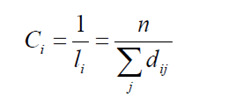
\includegraphics[width=4.8cm,height=2.3cm]{figures/closeness}
\centering
\caption{Closeness centrality}
\label{fig:closeness}
\end{figure}

\begin{sloppypar}
Pre každý uzol sa stanoví hodnota closeness centrality. Hodnoty closeness centrality sú blízke notmálnemu rozdeleniu, v ktorom 95\% populácie dát patrí do intervalu ${\big[ \mu - 2\cdot\sigma, \mu + 2\cdot\sigma \big]}$
\end{sloppypar}

Leadri ležia na hornom chvoste distribučnej funkcie, a teda horný interval použijeme pre identifikovanie leadrov. A teda uzly, ktoré majú väčšiu hodnotu closeness centrality ako krajná hodnota tohto intervalu, sú identifikovaní ako leadri.

\subsection{Outermost}
Podobne ako pri role \textit{Leader} pre identifikovanie outermostov sa využíva metrika closeness centrality. Outermosti budú ležať však na spodnom chvoste distribučnej funkcie closeness centrality.

A tak teda uzlyy, ktoré majú hodnotu closeness centrality nižšiu ako ${\big[ \mu - 2\cdot\sigma \big]}$, sú outermosti.

\subsection{Mediator}
Rolu mediator zastávajú tí jednotlivci, ktorí spájajú viacero komunít a sú tzv. spojmy medzi komunitami. 


Pre identifikáciu mediátorov sa definujú metriky založené na metrike betweeness centrality a to:  \textit{LBetweeness - LBC} a \textit{CBetweeness - CBC} a ďalej metriky, ktoré vyjadrujú koľko rozdielnych komunít uzol spája: \textit{DSCount} a \textit{DSPair}.


\subsubsection{LBeweeness}


\textbf{LPath} - Pred definíciou LBetweeness je potrebné definovať LPath a to nasledovne: \textit{LPath} je množina všetkých najkratších ciest medzi lídrami dvoch rozdielnych komunít. 

\begin{figure}[H]
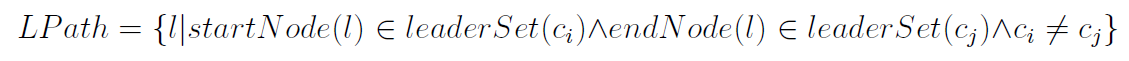
\includegraphics[width=16.5cm,height=1.1cm]{figures/lpath}
\caption{Def: LPath}
\end{figure}

{\setlength{\parindent}{0cm}
\begin{sloppypar}
\textbf{LBetweeness} centralita pre uzol \textit{v} - \textit{LBX(v)} je počet jedinečných LPath ktoré obsahujú \textit{v}. 


Ak pre každú cestu p  ${x \in}$ \textit{LPath} definujeme \textit{${I_l}$(p, v) = 1} ak \textit{v} leží na \textit{p}, inak \textit{${I_l}$(p, v) = 0} potom:
\end{sloppypar}
}
 

\begin{figure}[H]
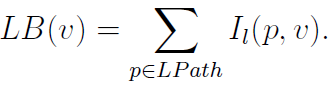
\includegraphics[width=5cm,height=1.3cm]{figures/lbetweenes}
\centering
\caption{Def: LBetweeness}
\end{figure}

\subsubsection{CBetweeness}
\begin{sloppypar}
CBetweeness počíta počet najkratších ciest medzi rozdielnymi komunitami. \textit{${s_p}$} a \textit{${e_p}$} označujú štartovací a koncový uzol najkratšej cesty \textit{p} . Taktiež \textit{${c_v}$} označuje komunitu, do ktorej uzol \textit{v} patrí. Množina všetkých najkratších ciest, ktoré spájajú rozdielne komunity:  
\textit{${CPaths = \{ p | {c_s}_p \neq {c_e}_p} \}$}. Taktiež definujeme ${I_p(p, v)}$ = 1 ak \textit{v} leží na ceste \textit{p} a 0 keď neleží.

\begin{figure}[H]
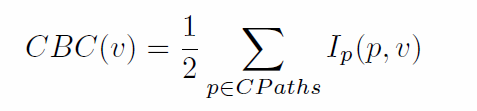
\includegraphics[width=6.5cm,height=1.7cm]{figures/cbetweeness}
\centering
\caption{Def: CBetweeness}
\end{figure}


\subsubsection{Normalizovaná CBetweeness}
Pravdepodobnosť nájdenia viac viditeľných mediátorov vo väčších komunitách je väčšia v porovnaní s menšími komunitami. Táto situácia sa stáva, pretože vo väčších komunitách je pochopiteľne viac uzlov, čo vedie k viacerým najkratším cestám medzi nimi. Pre kompenzáciu tohoto efektu je definovaná normalizovaná verzia \textit{CBC}: 


\begin{figure}[H]
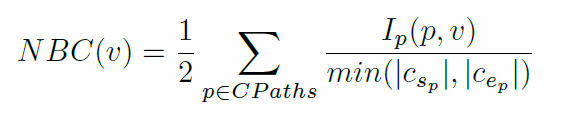
\includegraphics[width=6.5cm,height=1.7cm]{figures/normalizedCBC}
\centering
\caption{Def: Normalizovaná verzia CBC}
\end{figure}




\end{sloppypar}


\begin{sloppypar}
Navrhnuté metriky \textit{CBC} a \textit{LBC} sú nevyhnutné pre identifikovanie mediátorov, ale nie sú dostatočné. Napríklad pre sieť pozostávajúcu z desiatich komunít a dvoch mediátorov \textit{${M_1}$}
a \textit{${M_2}$}, kde oba ležia na sto najkratších cestách medzi komunitami majú oba rovnaké hodnoty \textit{CBC}. Kdežto \textit{${M_1}$} spája dve rozdielne komunity, kým \textit{${M_2}$} spája všetkých 10. Pri takomto scenári \textit{${M_2}$} spája komunity viac globálne a mal by byť skôr posudzovaný ako mediátor ako \textit{${M_1}$}. A tak \textit{${SSRM}$} definuje tzv. metriku \textbf{skóre rozmanitosti}, ktorá označuje rozdielne komunity, ktoré sú prepojené cez uzol.
\end{sloppypar}


\subsubsection{Skóre rozmanitosti}
\begin{sloppypar}
Táto metrika ukazuje koľko rozdielnych komunít je spojených cez špecifický uzol \textit{v}. Túto metriku definujeme v dvoch variantach:

\begin{enumerate}
\item 

\textbf{DSCount} - je definovaný ako počet rozdielnych komunít, ktoré sú spojené daným uzlom. Nech \textit{${I_d}({c_i}, v)$} = 1 ak \textit{${\exists p \in CPaths: {s_p} \in {c_i} \wedge	v \in p}$}. Potom DSScount uzla \textit{v} je definované ako:

\begin{figure}[H]
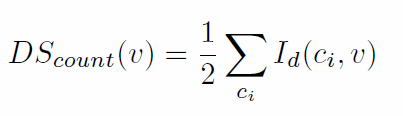
\includegraphics[width=6.5cm,height=1.7cm]{figures/dscount}
\centering
\caption{Def: DSCount}
\end{figure}


\item \textbf{DSPair} - Skóre rozmanitosti môže byť definované ako počet párov komunít, ktoré majú najmenej jednu najkratšiu cestu medzi ich členmi, ktoré prechádzajú uzlom \textit{v}. Definujeme  \textit{${I_d}({c_i},{c_j}, v)$} = 1 ak \textit{${\exists p \in CPaths: {s_p} \in {c_i} \wedge {e_p} \in {c_j} \wedge	v \in p}$}





\begin{figure}[H]
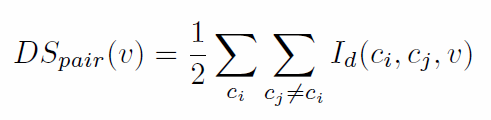
\includegraphics[width=6.5cm,height=1.7cm]{figures/dspair}
\centering
\caption{Def: DSPair}
\end{figure}

\end{enumerate}
\end{sloppypar}

Aj keď viac mediátorov môže mať rovnaké hodnoty jednotlivých metrík, 
môžu sa odlišovať napríklad v počte komunít, ktoré spájajú. SSRM to berie do úvahy a definuje tzv. \textit{mediacy score} ako násobok normalizovanej CBetweeness a skóra rozmanitosti:

\begin{figure}[H]
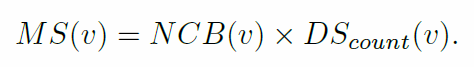
\includegraphics[width=10.5cm,height=1.7cm]{figures/mediacyscore}
\centering
\caption{Def: DSPair}
\end{figure}


\section{Prehľad systému}

\subsection{Konštrukcia siete}
Rozdiel medzi prísupom rôznych štúdií a mojím prístupom pri konšrukcii grafu z emailového dataetu je v konštrukcii komunikačnej siete. Ako základnú stavebnú jednotku siete som si zvolila \textbf{konverzáciu}. Konverzácia je súbor mailov, ktorá začína jediným mailom, obsahuje najmenej 2 emaily a dvoch rôznych odosielateľov. Vrcholom siete (grafu) sa teda stane užívateľ, ktorý bol ako odosielateľ aspoň v jednej takejto konverzácii. Hrana medzi užívateľmi je zostrojená medzi užívateľmi, ktorí boli spolu v jednej konverzácii ako odosielatelia. 

\subsection{Pre-processing}
Pre extrakciu dát z emailového účtu som použila separátnu aplikáciu \cite{5}, ktorá obsahuje konektor pre pripojenie k rôznym emailovým klientom(MS Outlook, Thunderbird) alebo sa pripojí cez IMAP alebo Gmail. Výstupom aplikácie je XML súbor (dataset) pripravný pre ďalšie používanie. Obsahuje prvky\textit{MessageId, Sender, Sent, Subject, InReplyTo, Recipient, Type(CC, To)}, ale neobsahuje telo emailu, ani prílohy.

Po tomto predpripravní dát z individuálneho emailového účtu môže byť súbor  naimportovaný do aplikácie.

\subsection{Import dát}
XML súbor je analyzovaný uloženou procedúrou, ktorá rozparsuje emailové dáta na jednodlivé entity - \textit{Users, EmailMessages EmailRecipients} a \textit{Conversations} a uloží ich do SQL databázy.

\subsection{Analýza}


\newpage
\begin{thebibliography}{99}
	\bibitem{1} Guanting Tang, Jian Pei, and Wo-Shun Luk: \textit{Email Mining: Tasks, CommonTechniques, and Tools}
	\bibitem{2} Xiaoyan Fu: \textit{Visualization and Analysis of Email Networks}
	\bibitem{3} J. Diesner, T. L. Frantz, and K. M. Carley: \textit{Communication networks
from the enron email corpus it’s always about the people. E 	nron is
no different}
	\bibitem{4} A. Chapanond, M. S. Krishnamoorthy, and B. Yener,  \textit{Graph Theoretic and Spectral Analysis of Enron Email Data }
	\bibitem{5} TeamNETData, \textit{http://inflex.cz:8075/TeamNETdata/}
	\bibitem{6} N. Crossley, E. Bellotti, G. Edwards, M. G. Everett, J. Koskinen, M. Tranmer,  \textit{Social network analysis for Ego-Nets}	
	\bibitem{7} Petr Kovář, \textit{Úvod do Teorie grafů} - skripta VŠB 
	\bibitem{8} M.E.J. Newman, \textit{The structure and function of complex networks}
	\bibitem{9} Afra Abnar, Mansoureh Takaffoli, Reihaneh Rabbany, Osmar R. Zaıane \textit{SSRM: Structural Social Role Miningfor Dynamic Social Networks}
	\bibitem{10} Zehnalová, Horák, Kudělka \textit{Email Conversation Network Analysis: Work Groups
and Teams in Organizations}
	\bibitem{11}
	\bibitem{12}
	\bibitem{13}
\end{thebibliography}



\end{document}
